%!Mode::"UTF-8"
\documentclass[12pt]{article}

% 页面设置
\usepackage{geometry}
\geometry{left=2.5cm, right=2.5cm, top=2.5cm, bottom=2.5cm}
\usepackage{graphicx}
\usepackage{ctex}
\usepackage{fontspec}
\usepackage{setspace}

% 字体设置
\setmainfont{Times New Roman}
\setCJKmainfont{SimSun}
\setCJKsansfont{SimHei}

% 表格设置
\usepackage{makecell}
\newcommand{\addcell}[2][4]{\makecell{\zihao{#1}\textsf{#2}}}
\usepackage{titlesec}
\usepackage{booktabs}
\usepackage{tabularx}

% 设置图注、表注
\usepackage{caption}
\usepackage{bicaption}
\captionsetup{labelsep=quad, font={small, bf}, skip=2pt}
\DeclareCaptionOption{english}[]{
    \renewcommand\figurename{Fig.}
    \renewcommand\tablename{Table}
}
\captionsetup[bi-second]{english}

% 设置页眉
\usepackage{fancyhdr}
\pagestyle{fancy}
\fancypagestyle{preContent}{
    \fancyhead[L]{\zihao{-5} 物理化学实验}
    \fancyhead[C]{\zihao{-5} 实验十一\ \ 量子化学计算方法及Gaussian程序的使用}
    \fancyhead[R]{\zihao{-5} 1800011828\ 王宇哲}
}
\pagestyle{preContent}

%	设置首页页眉页脚
\fancypagestyle{plain}{
	\fancyhead[L]{\zihao{-5} 物理化学实验}
	\fancyhead[C]{\zihao{-5} 实验十一\ \ 量子化学计算方法及Gaussian程序的使用}
	\fancyhead[R]{\zihao{-5} 1800011828\ 王宇哲}
	\cfoot{}
}

% 设置标题格式
\titleformat*{\section}{\zihao{4}\sffamily}
\titleformat*{\subsection}{\zihao{-4}\sffamily}
\titleformat*{\subsubsection}{\zihao{-4}\sffamily}
\titlespacing*{\section}{0pt}{10pt}{10pt}
\titlespacing*{\subsection}{0pt}{10pt}{5pt}
\titlespacing*{\subsubsection}{0pt}{10pt}{5pt}

% 设置引用格式
\usepackage[super,round,comma,compress]{natbib}

\usepackage{amsmath}
\usepackage{amssymb}

\begin{document}
    % 标题页
    \begin{titlepage}
    	% 页眉
    	\thispagestyle{plain}
        % 图片
        \begin{figure}[h]
            \centering
            \includegraphics{pku.png}
        \end{figure}
        \vspace{24pt}
        % 标题
        \centerline{\zihao{-0} \textsf{物理化学实验报告}}
        \vspace{40pt} % 空行
        \begin{center}
            \begin{tabular}{cp{14.1cm}}
                % 题目
                \addcell[2]{题目:\ } & \addcell[2]{量子化学计算方法及Gaussian程序的使用} \\
                \cline{2-2}
            \end{tabular}
        \end{center}
        \vspace{20pt} % 空行
        \begin{center}
            \doublespacing
            \begin{tabular}{cp{5cm}}
                % 姓名
                \addcell{姓\phantom{空格}名:\ } & \addcell{王宇哲} \\
                \cline{2-2}
                % 学号
                \addcell{学\phantom{空格}号:\ } & \addcell{1800011828}\\
                \cline{2-2}
                % 组别
                \addcell{组\phantom{空格}别:\ } & \addcell{11组} \\
                \cline{2-2}
                % 实验日期
                \addcell{实验日期:\ } & \addcell{2020.9.23}\\
                \cline{2-2}
                % 室温
                \addcell{室\phantom{空格}温:\ } & \addcell{296.65\ K}\\
                \cline{2-2}
                % 大气压强
                \addcell{大气压强:\ } & \addcell{102.17\ kPa}\\
                \cline{2-2}
            \end{tabular}
            \begin{tabular*}{\textwidth}{c}
                \\ % 这是空行
                \\ % 这是空行
                \\ % 这是空行
                \\ % 这是空行
                \hline % 分割线
            \end{tabular*}
        \end{center}
        % 摘要
        \textsf{摘\ \ 要}\ \ 本实验通过量子化学计算方法,利用Gaussian03W软件对指定分子进行量化计算,得到了正丁醇的偶极矩、萘和甘菊环的能量差$\Delta E_{total}=-1.4\times10^{2} \ \ {\rm kJ \cdot mol^{-1}} $,O$_{2}$的键能$E_{bond}=522\ \ {\rm kJ \cdot mol^{-1}}$,比较了不同分子中羰基的强弱,对不同计算方法和基组进行了对比,从而初步了解了量化计算的基本原理和方法。
        \\
        \\
        % 关键字
        \textsf{关键词}\ \ 量子化学计算;Gaussian03W;GaussView;基组
    \end{titlepage}

    \section{引言}
	量子化学利用量子力学理论处理与化学相关的问题,通过对于电子和核量子行为的描述,原则上能够处理几乎所有化学现象,包括密度和颜色等经典物理量、各类光电子能谱等明显具有量子特性的量以及原子尺度下电子密度的分布等实验上难以测量的量。为解决实际问题,量子化学需要在精度和效率中做权衡,其重要研究内容就是如何发展适宜的方法、程序,近似求解方程,从而应用于实际体系。\par
	随着相关研究的进展,量子化学领域发展了多种求解电子和核运动方程的方法。根据近似程度,量子化学方法可大致分为三大类,即包含MNDO、AM1、PM3等的半经验方法、包含HF、MPn等的从头算方法和基于电荷密度自洽的DFT方法。基于以上方法,开发了量子化学的商用软件Gaussian程序,具有各种近似解量子力学方程的功能。\par
	本次实验利用GaussView软件生成和优化指定分子,利用Gaussian03W软件对指定分子进行量化计算,得到指定分子的偶极矩、能量、化学键键能、不同分子中羰基强弱等实验数据,并对不同的计算方法和基组进行了比较。通过本次实验,可以初步了解量子化学计算的基本原理和方法,学习使用Gaussian软件;通过计算手段,定量比较官能团稳定性等化学性质,从而更充分地认识到量化计算的重要意义。
               
\vbox{}        
    \section{实验部分}
    	\subsection{软件程序}
    	GaussView和Gaussian09W
    	
    	 \subsection{实验内容}
			\subsubsection{计算正丁醇分子偶极矩}
			使用GaussView软件生成正丁醇分子;分别使用AM1、HF、B3LYP方法进行结构优化 (opt) ,其中HF和B3LYP方法选择3-21G和6-31G(d)两种基组;分别从结果文件中记录偶极矩值和计算时间,对实验结果和文献值加以对比。
			\subsubsection{计算萘和甘菊环分子能量}
			分别使用GaussView软件生成萘 (naphthalene) 和甘菊环 (azulene) 分子;使用B3LYP/6-31G(d)进行结构优化和频率计算(opt-freq);分别从结果文件中记录两个分子的总能量、电子能、平动能、转动能和振动能;计算两分子的能量差。
			\subsubsection{计算O$_{2}$分子键能}
			分别使用GaussView软件生成O$_{2}$分子和O原子,自旋多重度均为3;使用B3LYP/6-31G(d)(Unrestricted)进行结构优化(opt);分别从结果文件中记录O$_{2}$分子和O原子的能量;计算能量差,得到O$_{2}$分子的键能。
			\subsubsection{比较乙酸、乙醛、丙酮羰基强弱}
			分别使用GaussView软件生成乙酸、乙醛、丙酮分子;使用B3LYP/6-31G(d)进行结构优化和频率计算(opt-freq);分别从结果文件中记录3个分子羰基的振动基频,分析3个分子中羰基的强弱。
			\subsubsection{计算Zn、Cu原子吸收峰波长}
			分别使用GaussView软件生成Zn、Cu原子; 分别使用B3LYP/6-311++G(2d,2p)和B3LYP/cc-pVTZ进行TDDFT计算,从结果文件中记录两原子的第一激发态能量和对应吸收峰波长。
    	
\vbox{}  
	 \section{数据与结果}
 		\subsection{实验数据记录及处理}
 		            \subsubsection{计算正丁醇分子偶极矩}
 		使用GaussView画出正丁醇分子优化后的三维结构如\textbf{图1}所示。\par
 		 \begin{figure}[h]
 			\centering
 			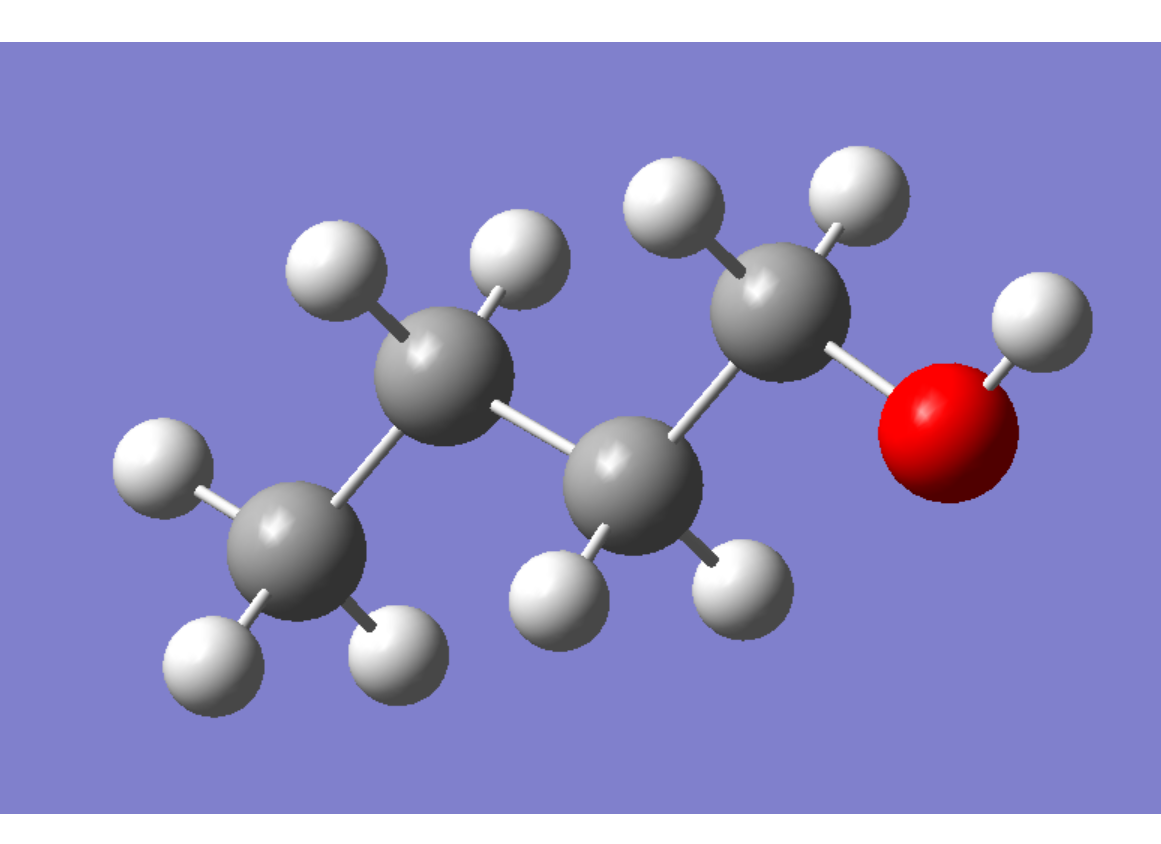
\includegraphics[width=0.5\textwidth]{1.png}
 			\bicaption{正丁醇分子优化后的结构}{Optimized structure of n-butanol molecule}
 		\end{figure}
 		计算正丁醇偶极矩的相关数据如\textbf{表1}所示。
 		  \begin{table}[h]
 			\centering
 			\zihao{5}
 			\bicaption{正丁醇的偶极矩$\mu$}{Dipole moment $\mu$ of n-butanol molecule}
 			\begin{tabular}{cccc}
 				\toprule
 				序号 & 方法及基组 & 偶极矩$\mu$ / D & 计算时间$t$ / s \\
 				\midrule
 				1 & AM1 & 1.5211 & 3.0 \\
 				2 & HF / 3-21G & 1.8715 & 7.0 \\
 				3 & HF / 6-31G(d) & 1.6940 & 31.0 \\
 				4 & B3LYP / 3-21G & 1.6277 & 61.0 \\
 				5 & B3LYP / 6-31G(d) & 1.5223 & 110.0 \\
 				\bottomrule
 			\end{tabular}
 		\end{table}
 	
\vbox{}
 		 \subsubsection{计算萘和甘菊环分子能量}
 		 	使用GaussView画出萘和甘菊环分子优化后的三维结构如\textbf{图2}所示,其中(a)为萘分子,(b)为甘菊环分子。\par
 		 	
 		 \begin{figure}[h]
 		 	\centering
 		 	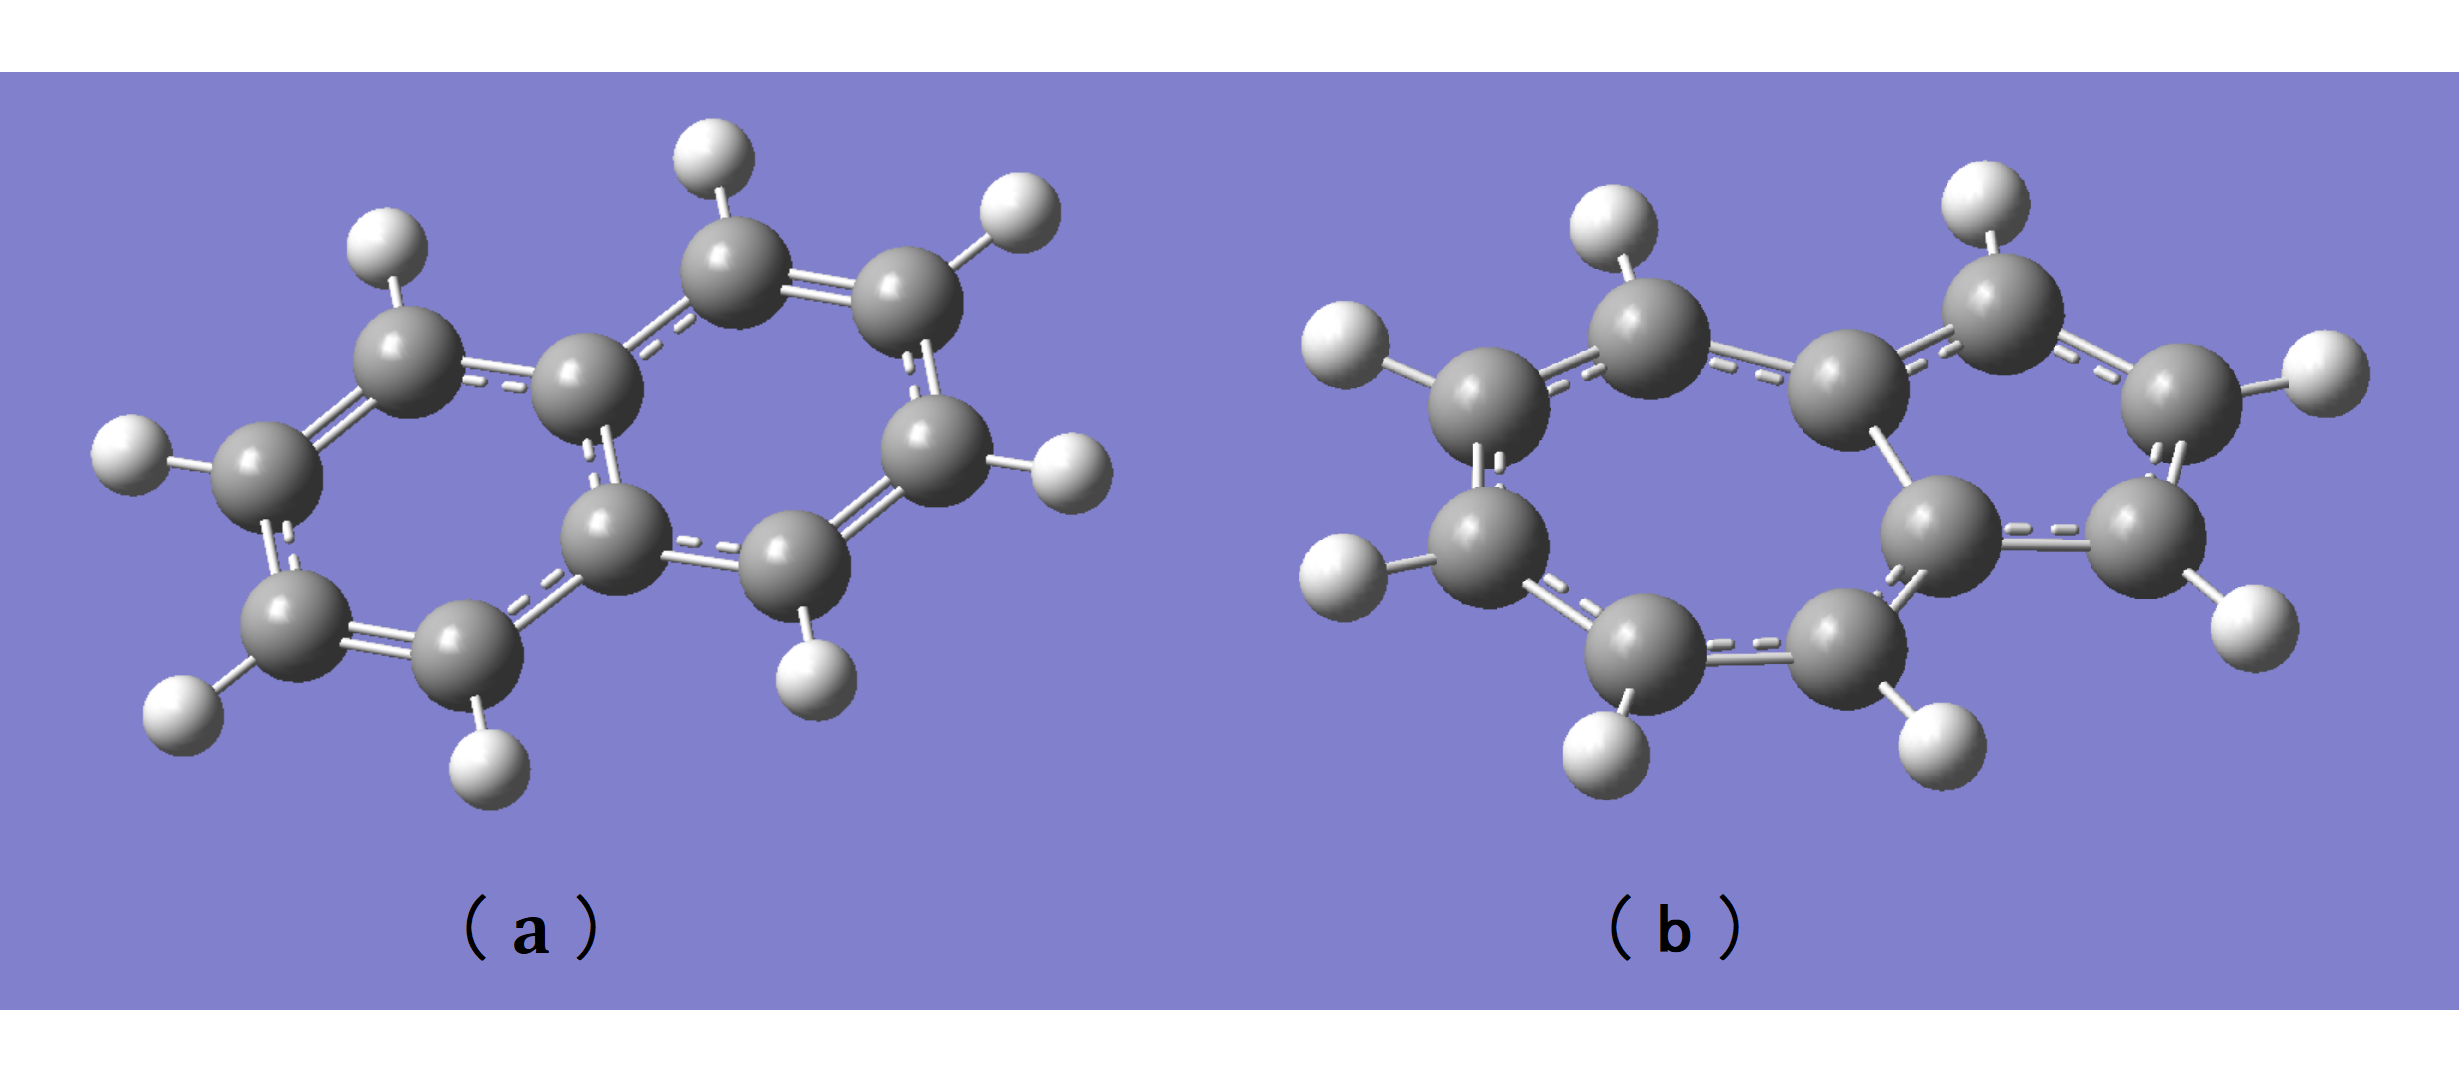
\includegraphics[width=0.7\textwidth]{2.png}
 		 	\bicaption{萘和甘菊环分子优化后的结构}{Optimized structure of naphthalene and azulene molecules}
 		 \end{figure}
 	 
 		计算萘和甘菊环分子能量的相关数据以及处理结果如\textbf{表2}所示;表中$E_{trans}$、$E_{rot}$、$E_{vib}$、$E_{elec}$、$E_{total}$分别为分子的平动能、转动能、振动能、电子能和总能量,且有$$ E_{total}=E_{trans}+E_{rot}+E_{vib}+E_{elec} $$ 
 		通过单位换算$ 1\ \ {\rm a.u.}=2625.50 \ \ {\rm kJ \cdot mol^{-1}} $及$1\ \ {\rm kcal \cdot mol^{-1}}=4.18585\ \ {\rm kJ \cdot mol^{-1}}$,计算得到的能量已被转换成标准单位。
 		  \begin{table}[h]
 			\centering
 			\zihao{5}
 			\bicaption{萘和甘菊环分子的能量}{Energy of naphthalene and azulene molecules}
 			\begin{tabular}{cccccccc}
 			\toprule
 				序号 & 方法及基组 & 分子 & \thead[c] {$E_{trans}$ \\ / $ \rm kJ \cdot mol^{-1} $} & \thead[c]{$E_{rot}$ \\ / $ \rm kJ \cdot mol^{-1} $} & \thead[c]{$E_{vib}$ \\ / $ \rm kJ \cdot mol^{-1} $} & \thead[c] {$E_{elec}$ \\ / $ \rm kJ \cdot mol^{-1} $} & \thead[c]{$E_{total}$ \\ / $ \rm kJ \cdot mol^{-1} $} \\
 			\midrule
 			1 & B3LYP / 6-31G(d) & 萘 & 3.72 & 3.72 & 398.71 & -1.01316$\times10^{6}$ & -1.01275$\times10^{6}$ \\
 			2 & B3LYP / 6-31G(d) & 甘菊环 & 3.72 & 3.72 & 396.14 & -1.01302$\times10^{6}$ & -1.01261$\times10^{6}$ \\
 			\bottomrule
 			\end{tabular}
 		\end{table}\par
 	计算两分子的能量差$$\Delta E_{total}=E_{total}({\rm nap})-E_{total}{\rm (azu)=-1.4\times10^{2} \ \ kJ \cdot mol^{-1} }$$
 	
 		\subsubsection{计算O$_{2}$分子键能}
 			使用GaussView画出O$_{2}$分子优化后的三维结构如\textbf{图3}所示。\par
 		\begin{figure}[h]
 			\centering
 			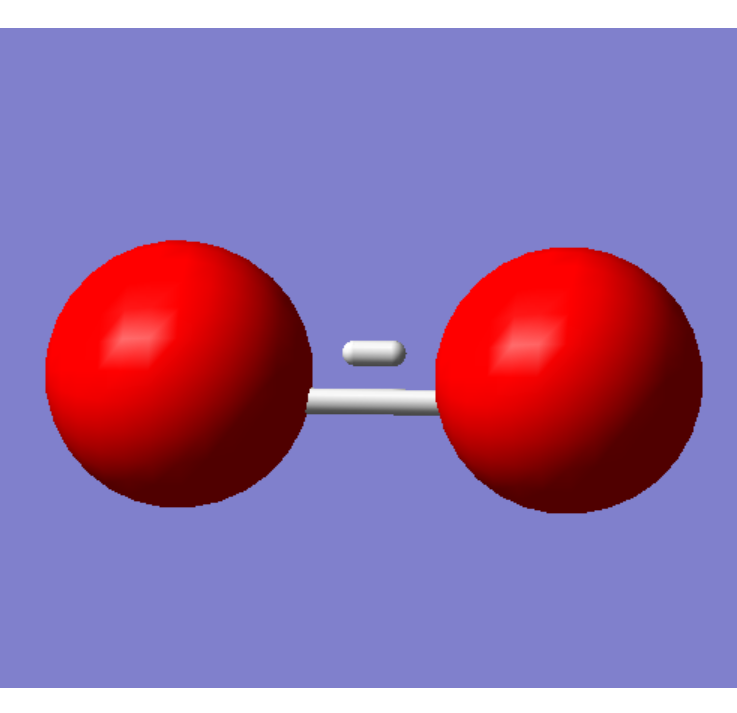
\includegraphics[width=0.4\textwidth]{3.png}
 			\bicaption{O$_{2}$分子优化后的结构}{Optimized structure of O$_{2}$ molecule}
 		\end{figure}
 		计算O$_{2}$分子键能的原始数据如\textbf{表3}所示。\par
 		  \begin{table}[h]
 			\centering
 			\zihao{5}
 			\bicaption{O$_{2}$ 分子的键能}{Bond energy of O$_{2}$ molecule}
 			\begin{tabular}{cccc}
 				\toprule
 					序号 & 方法及基组 & 物种 & $E$ / $\rm kJ \cdot mol^{-1} $ \\
 				\midrule
 				1 & B3LYP / 6-31G(d) \ \ (Unrestricted) & O$_{2}$ & $-3.94665 \times 10^{5}$ \\
 				2 & B3LYP / 6-31G(d) \ \ (Unrestricted) & O & $-1.97072 \times 10^{5}$ \\
 				\bottomrule
 			\end{tabular}
 		\end{table}
 	根据\textbf{表3}数据,计算O$_{2}$分子键能$$E_{bond}=2E({\rm O})-E{\rm (O_{2})}=522\ \ {\rm kJ \cdot mol^{-1}}$$
 	
 		\subsubsection{比较乙酸、乙醛、丙酮羰基强弱}
 			使用GaussView画出乙酸、乙醛、丙酮分子优化后的三维结构如\textbf{图4}所示,其中(a)为乙酸,(b)为乙醛,(c)为丙酮。\newpage
 		
 		\begin{figure}[h]
 			\centering
 			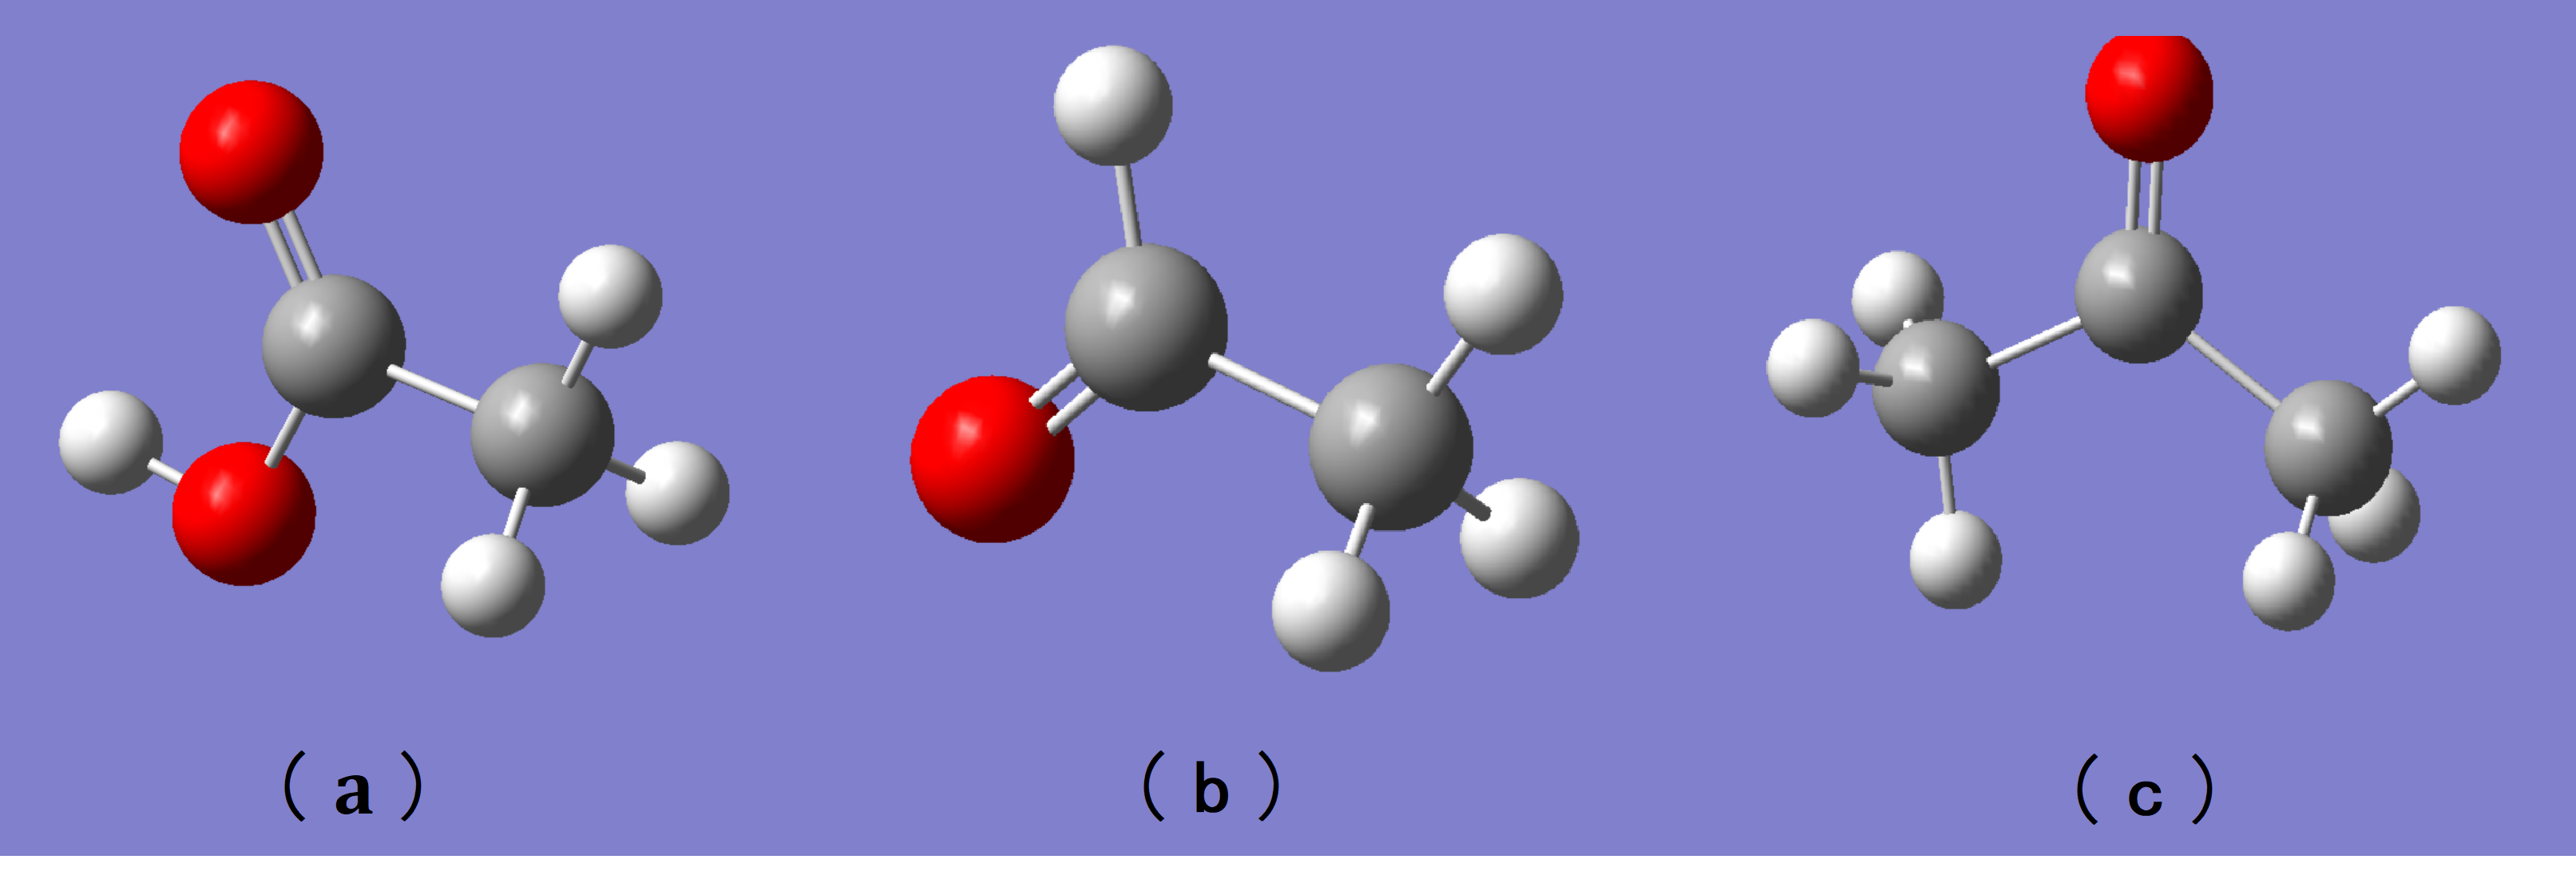
\includegraphics[width=0.8\textwidth]{4.png}
 			\bicaption{乙酸、乙醛、丙酮分子优化后的结构}{Optimized structure of acetic acid, acetaldehyde and acetone molecules}
 		\end{figure}
 		
 		计算乙酸、乙醛、丙酮分子羰基振动基频的相关数据如\textbf{表4}所示。
 		  \begin{table}[h]
 			\centering
 			\zihao{5}
 			\bicaption{乙酸、乙醛、丙酮分子羰基强弱}{Carbonyl strength of acetic acid, acetaldehyde and acetone molecules}
 			\begin{tabular}{cccc}
 				\toprule
 				序号 & 方法及基组 & 分子 & 羰基振动基频$\tilde{\nu}$ / ${\rm cm^{-1}}$ \\
 			\midrule
 			1 & B3LYP / 6-31G(d) & 乙酸 & 1858.11 \\
 			2 & B3LYP / 6-31G(d) & 乙醛 & 1837.45 \\
 			3 & B3LYP / 6-31G(d) & 丙酮 & 1822.03 \\
 			
 				\bottomrule
 			\end{tabular}
 		\end{table}
 	
 		 \subsubsection{计算Zn、Cu原子吸收峰波长}
 		计算Zn、Cu原子第一激发态能量和对应吸收峰波长的相关数据如\textbf{表5}所示。
 		  \begin{table}[h]
 		  	\setlength{\belowcaptionskip}{-0.73pt}
 			\centering
 			\zihao{5}
 			\bicaption{Zn、Cu原子的第一激发态能量和吸收峰波长}{The first excited state energy and absorption peak wavelength of Zn, Cu atoms}
 			\begin{tabular}{ccccc}
 				\toprule
 				序号 & 方法及基组 & 原子 & 第一激发态能量$E$ / eV & 吸收峰波长$\lambda$ / ${\rm nm}$ \\
 			\midrule
 			1 & B3LYP / 6-311++G(2d, 2p) & Zn & 5.6577 & 219.14 \\
 			2 & B3LYP / cc-pVTZ & Zn & 5.6213 & 220.56 \\
 			3 & B3LYP / 6-311++G(2d, 2p) & Cu & 1.5572 & 796.18 \\
 			4 & B3LYP / cc-pVTZ & Cu & 1.4055 & 882.11 \\
 				\bottomrule
 			\end{tabular}
 		\end{table}
 	
 		\subsection{实验结果及分析}

 		\subsubsection{计算正丁醇分子偶极矩}
 		本实验通过使用不同方法和基组、使用Gaussian软件进行结构优化(opt),从结果文件中得到偶极矩的计算值和计算时间如\textbf{表1};\par 比较\textbf{表1}中不同方法和基组的计算时间$t$,可以发现计算所消耗的时间
 
 			$$ \setlength{\abovedisplayskip}{-3pt} \rm B3LYP/6-31G(d) > B3LYP/3-21G > HF/6-31G(d) > HF/3-21G > AM1 $$
 
 	即B3LYP方法耗时最多,HF方法次之,AM1方法耗时最少;对于B3LYP和HF方法,基组增大,计算耗时也显著增加;\par
 		比较偶极矩$\mu$的计算值与参考值
 		\citealp{dean1992lange} 
 		$\mu=1.66\ \ {\rm D}$,可以发现计算正丁醇偶极矩的精度
 	
 		$$\setlength{\abovedisplayskip}{-3pt}\rm	B3LYP/3-21G \approx HF/6-31G(d) > B3LYP/6-31G(d) \approx AM1 > HF/3-21G $$
 	其中AM1和B3LYP方法计算值偏小,HF方法计算值偏大。
 		
 		\subsubsection{计算萘和甘菊环分子能量}
 		本实验通过使用Gaussian软件进行结构优化和频率计算(opt-freq),从结果文件中得到萘和甘菊环分子的各项能量如\textbf{表2},算得两分子能量差$\Delta E_{total}=-1.4\times10^{2} \ \ {\rm kJ \cdot mol^{-1} } $;\par
 		比较\textbf{表2}中萘和甘菊环分子的各项能量,可以发现总能量中不同能量项的贡献$$\vert E_{elec}\vert \gg E_{vib}>E_{trans}\approx E_{rot} $$\par
萘分子总能量低于甘菊环分子;分析\textbf{表2}数据,两分子平动能$E_{trans}$、转动能$E_{rot}$几乎完全相同,萘的振动能$E_{vib}$甚至略微高于甘菊环,而电子能$E_{elec}$则有较大差别,故该能量差异主要来自萘分子较低的电子能$E_{elec}$。
 		\subsubsection{计算O$_{2}$分子键能}
 		本实验通过使用Gaussian软件进行结构优化(opt),从结果文件中得到相关数据如\textbf{表3},算得O$_{2}$的键能$E_{bond}=522\ \ {\rm kJ \cdot mol^{-1}}$。\par
 		\subsubsection{比较乙酸、乙醛、丙酮羰基强弱}
 		本实验通过使用Gaussian软件进行结构优化和频率计算(opt-freq),从结果文件中得到乙酸、乙醛、丙酮分子的羰基振动基频如\textbf{表4};\par
 			比较\textbf{表4}中乙酸、乙醛、丙酮分子的羰基振动基频,有$$\tilde{\nu} {\rm (acetic \ \  acid)}>\tilde{\nu} {\rm (acetaldehyde)}>\tilde{\nu}{\rm (acetone)}$$根据以上结果,可以判断三个分子中羰基的强弱顺序为:乙酸 > 乙醛 > 丙酮。
 		\subsubsection{计算Zn、Cu原子吸收峰波长}
 		本实验通过使用Gaussian软件进行TDDFT计算,从结果文件中得到Zn、Cu两原子的第一激发态能量和对应吸收峰波长如\textbf{表5};相比实验值\citealp{Bast2009,Konecny2019}
 		$$E_{\rm Zn}=5.80 \ \ {\rm eV}\ \ \ \ \ \ \ E_{\rm Cu}=1.39\ \ {\rm eV}$$
 		可以发现cc-pVTZ和6-311++G(2d, 2p)两个基组计算Zn的第一激发态能量的精度相近,均略小于实验值;而基组cc-pVTZ计算Cu的第一激发态能量十分接近实验值,精度远高于基组6-311++G(2d, 2p)。
 		

 	
\vbox{}  	
 	 \section{讨论与结论}
		\subsection{实验讨论}
 			\subsubsection{同一分子结构优化得到不同构象的原因分析}
 	 在对正丁醇分子进行结构优化并计算偶极矩时,组内有成员计算结果与参考值有明显的差异,进一步分析发现该组员使用Gaussian程序进行结构优化所得构象明显非能量最低构象。经组内讨论,分析可能的原因是在GaussView中生成正丁醇分子的初始构象不同,导致通过梯度下降法进行结构优化的结果落入不同的局部极小,从而获得不同的构象。查阅相关文献了解到,输入的初始结构对结构优化的计算结果有很大影响,对于较为复杂的体系,初始结构的轻微扰动常使结构收敛到不同的能量极小点,从而导致分子几何优化结果的重现性较差。\citealp{Williams_2007}\par
 	 在实际计算中,为避免结构优化落入局部极小,对于较为简单的分子,可以使用Gaussian进行势能面扫描,从而直观看出能量最小值所对应的分子构象;也可以使用Chem3D等软件对分子的初始结构进行预优化,再利用Gaussian程序进行计算,使得计算结果更大概率为能量全局最小;对于较复杂的体系,相关研究人员开发了粒子群优化(Particle Swarm Optimization)等方法\citealp{Call_2007}对体系进行全局能量最小化搜索,从而有效跳出局部极小,得到全局最小的结果。
 	 \subsubsection{量化计算方法和基组选取的讨论}
 	 在实际计算中,选取量化计算方法和基组既要考虑计算体系的情况,又要考虑算力、耗时和精度要求。本次实验可以发现,对于大多数体系,B3LYP等DFT方法的精度都显著高于半经验方法和HF等从头算方法,但其耗时也明显高于后两者;随着基组的增大,在一些体系上计算精度得到相当程度的提高,但计算耗时也大幅上升。因此,对于简单分子结构优化等精度要求不高的问题,可以使用精度较低的方法和较小的基组以节约计算时间;对于计算分子光谱等对精度要求较高的问题,则应当适当增大基组,否则所得结果很可能误差过大。
 	 \subsection{实验结论}
 	 本实验通过量子化学计算方法,利用Gaussian03W软件进行量化计算,得到了正丁醇分子的偶极矩、萘和甘菊环分子的各项能量、O$_{\rm 2}$分子的键能、乙酸、乙醛、丙酮分子中羰基的振动基频,并对不同的计算方法和基组进行了对比,从而初步了解了量子化学计算方法的基本原理、应用以及Gaussian程序的使用方法;通过对比,可发现量化计算所得结果与实验参考值及定性规律具有很好的一致性,充分证明了量化计算的可靠性与强大威力。\par
 	 作为成熟的量子化学商用软件,Gaussian程序内置了大量适用于不同量化计算领域的基组,而弥散函数、极化函数等的广泛使用使得量化计算方法与基组的选取具有相当程度的技巧性。本次实验初步探究了不同量化计算方法与基组的差异,而本实验中的计算体系如何选取最优的计算方法和基组,类似的经验性规律值得进一步学习、研究与思考。
 
 

   

\vbox{}  

\bibliographystyle{achemso}
\bibliography{cite}



\end{document}